\chapter{Authorization}
In this chapter are analyzed all the aspects that build the \textit{authorization} infrastructure in Istio Security. Moreover, a further analysis is done on the policies, ending with an in-depth analysis on the policy enforcement mechanism in order to understand how they are translated in firewall rules to enable/disable the communications between services.
\minitoc

\section{Architecture}
Istio Security gives the possibility to perform authorization for workload-to-workload and user-to-workload. Moreover, it supports any TCP protocols, in particular HTTP, HTTPS and gRPC. It is flexible, since custom conditions can be defined on Istio attributes and it uses only a single and simple beta API (\texttt{AuthorizationPolicy}) to store the policies and enforce the authorizations directly on the Envoy proxies.
In Fig.~\ref{fig:archauthz} a schematic description of the general authorization architecture is shown.

\begin{figure}[ht]
    \centering
    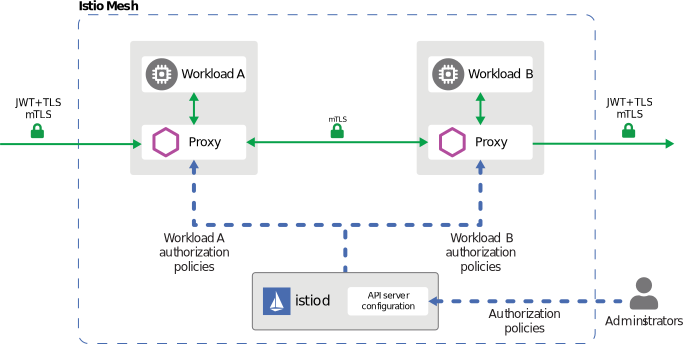
\includegraphics[width=0.9\textwidth]{chapters/images/chp3/arch-authz.png}
    \caption{, from Istio Docs}
    \caption[Istio Security's v1.6 authorization architecture]{Istio Security's v1.6 authorization architecture\\Source: \url{https://istio.io/v1.6/docs/concepts/security/authz.svg}}
    \label{fig:archauthz}
\end{figure}

More in details, once that an administrator applies an authorization policy (using the API server provided by \texttt{istiod}), the policy is split and sent to the interested workload. Here, Envoy takes the policy and runs an authorization controller that, based on the future request, evaluates the context with the policy and \texttt{DENY} or \texttt{ALLOW} the authorization. If no authorization policy is available for a particular workload, then the access control is disabled and all the requests are accepted. For multiple \texttt{AuthorizationPolicy}, the \texttt{DENY} takes precedence over the \texttt{ALLOW} and the specified policies are added by preserving the previously added ones (additively).

\section{Policies}
As already mentioned, the only way of defining custom policies is through the Istio API by using the \texttt{AuthorizationPolicy} kind in the \texttt{.yaml}. As an example, the following policy is chosen \cite{authzpolicy}:

\begin{lstlisting}
apiVersion: security.istio.io/v1beta1
kind: AuthorizationPolicy
metadata:
 name: httpbin
 namespace: foo
spec:
 selector:
   matchLabels:
     app: httpbin
     version: v1
 action: ALLOW
 rules:
 - from:
   - source:
       principals: ["cluster.local/ns/default/sa/sleep"]
   - source:
       namespaces: ["dev"]
   to:
   - operation:
       methods: ["GET"]
   when:
   - key: request.auth.claims[iss]
     values: ["https://accounts.google.com"]
\end{lstlisting}

\noindent This policy allows two sources (\texttt{cluster.local/ns/default/sa/sleep} service account and \texttt{dev} namespace) to access the workloads by using the \texttt{httpbin} app \texttt{v1} in the namespace \texttt{foo} when a JWT valid Token is used.

\noindent From this example can be extrapolated the structure of the text file:

\begin{itemize}
 \item \texttt{selector}: the target of the policy. In this example is everything that matches \texttt{httpbin} and has version \texttt{v1}.
 \item \texttt{action}: \texttt{ALLOW} or \texttt{DENY}.
 \item \texttt{rules}: when the action is triggered. Furthermore, other keywords are defined, such as \texttt{from} (to specify the source), \texttt{to} (for specifying the operations) and \texttt{when} (to specify the conditions needed).
\end{itemize}

In order to ensure that an allow policy won't bypass a deny one, the Envoy engine checks and evaluates first the deny ones. As another example, it can be added another policy that denies every access that is not from the namespace \texttt{foo}:

\begin{lstlisting}
apiVersion: security.istio.io/v1beta1
kind: AuthorizationPolicy
metadata:
 name: httpbin-deny
 namespace: foo
spec:
 selector:
   matchLabels:
     app: httpbin
     version: v1
 action: DENY
 rules:
 - from:
   - source:
       notNamespaces: ["foo"]
\end{lstlisting}

\noindent This second policy will be literally "added" to the first one, but since it is a deny policy it will be applied first. The resulting policy will be the intersection of the previously applied ones: as a result, only the source from namespace \texttt{foo} is allowed. 

Moreover, Istio allows custom conditions by using \texttt{when} in combination with the \texttt{key} values\footnote{See \url{https://istio.io/v1.6/docs/reference/config/security/conditions/}} that can be compatible with HTTP, TCP or both of them. For example, the policy can match only defined IP addresses in TCP or HTTP by using \texttt{source.ip} or even match in HTTP-only a defined JWT Token value, for example the audience (\texttt{request.auth.audiences}). The compatibility with TCP-only workload enables a restriction on some HTTP-only fields: 

\begin{itemize}
    \item \texttt{request\_principals}
    \item \texttt{hosts}
    \item \texttt{methods}
    \item \texttt{paths}
\end{itemize}

\noindent That cannot be used on TCP workloads. If, for some reasons, they are used, Istio will automatically ignore them. This is a pretty simple yet safe method.

Apart from custom conditions (that include the particular cases of \textit{allow-all} and \textit{deny-all}), Istio exploits the authenticated and unauthenticated identity. On one hand, in order to make a workload publicly accessible, the documentation specifies to not define the \texttt{source} section. On the other hand, to allow only authenticated users, it is necessary to set the \texttt{principals} section to "*". Since Istio uses mTLS for secure communication, some fields of the authorization policy conditionally require mTLS: \texttt{principals}, \texttt{namespaces}, \texttt{source.principal}, \texttt{source.namespace}, \texttt{connection.sni}.

\section{In-depth analysis: policy enforcement}
How Istio converts the \texttt{AuthorizationPolicy} YAML file into firewall rules or other rules to block or enable communications between services? 

\begin{figure}
    \centering
    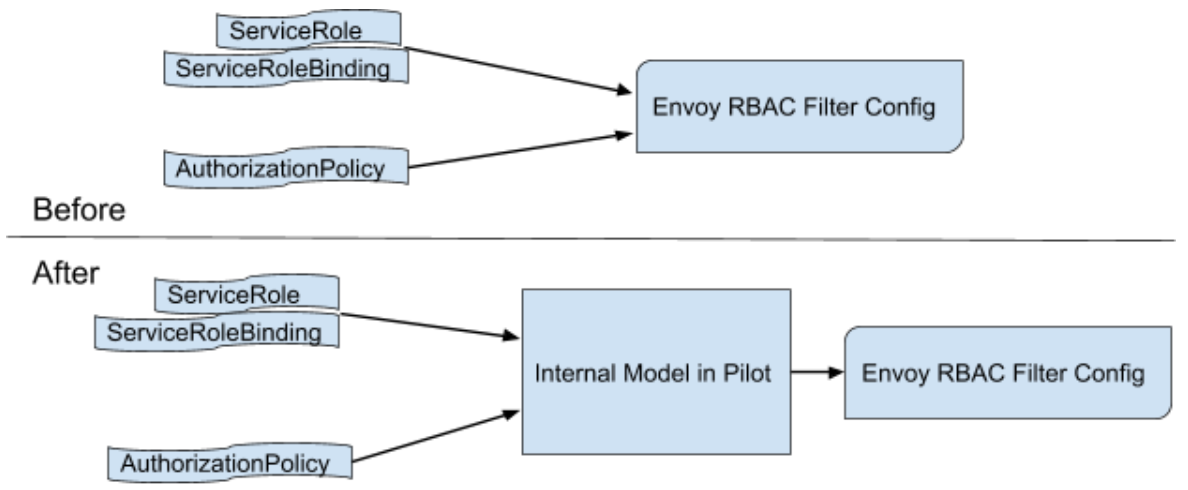
\includegraphics[width=0.9\textwidth]{chapters/images/chp3/before-after.png}
    \caption{Istio Security refactor with the internal model}
    \label{fig:int-rep}
\end{figure}


In the last year, Istio has undergone several changes. In the current version (v1.6) the policy is translated into an internal representation and then converted into an Envoy RBAC\footnote{Role-based access control, "[...] an approach to restricting system access to authorized users". Source: \url{https://en.wikipedia.org/wiki/Role-based_access_control}} Filter Config by using the Envoy API (Fig.~\ref{fig:int-rep}).
The old flow (Before) converts the Istio API directly to Envoy API in one step, while the new flow (After) converts it in two steps: 
\begin{enumerate}
    \item Convert the Istio API first to the internal model.
    \item Convert the internal model to the Envoy API.
\end{enumerate}

This refactor introduces some benefits regarding the coexistance of the old and new API (Alpha and Beta), like the possibility to write the code for converting the model to Envoy API once (it could be shared by both alpha and beta policy), making sure to have consistent behavior for both alpha and beta policy support. Furthermore, with this refactor it is only needed to convert beta policy to the internal model (which is much easier as it’s mostly a 1-1 mapping between the beta policy and the internal model).

\subsection{Istio API to Internal Model}

The first important thing to define is how the Istio API \texttt{AuthorizationPolicy} and the Internal Model are structured.
In the previous section, it has been covered the structure of the \texttt{AuthorizationPolicy}. The libraries for serialize/deserialize the YAML file are automatically built with Google's Protocol Buffer, as for the Authentication API (see \ref{protobuf}). The Istio API structure is pretty simple, it follows the YAML file and it is available on \href{https://github.com/istio/api/blob/release-1.6/security/v1beta1/authorization.proto}{GitHub}. In particular, the \textit{Rule} data structure is used to populate the Internal Model in order to be ready for the final conversion in Envoy RBAC filter API. This Internal Model is basically a high-level abstraction of the low-level Envoy RBAC filter API. It has the following structure:

\begin{lstlisting}

type Model struct {
	Permissions []Permission
	Principals  []Principal
}

type Permission struct {
	Services    []string // For backward-compatible only.
	Hosts       []string
	NotHosts    []string
	Paths       []string
	NotPaths    []string
	Methods     []string
	NotMethods  []string
	Ports       []int32
	NotPorts    []int32
	Constraints []KeyValues
}

type Principal struct {
	User          string // For backward-compatible only.
	Names         []string
	NotNames      []string
	Group         string // For backward-compatible only.
	Groups        []string
	NotGroups     []string
	Namespaces    []string
	NotNamespaces []string
	IPs           []string
	NotIPs        []string
	Properties    []KeyValues
}
\end{lstlisting}

\noindent Furthermore, it must be pointed out that is not saved or stored, it is only a temporary conversion of the Istio API policy that is waiting to be converted in RBAC filter API.
The Internal Model is built starting from the Istio API Rule, taken from the YAML in the \texttt{model.go} file by the following function:

\begin{lstlisting}[title=\href{https://github.com/istio/istio/blob/4e6e7f49375d84bb35ee614c6b7d38b6c2fd3e7b/pilot/pkg/security/authz/model/model.go\#L80-L148}{GitHub permalink}]
func New(r *authzpb.Rule, isIstioVersionGE15 bool) (*Model, error)
\end{lstlisting}

\noindent That literally builds a new model representing the authorization policy by adding the defined \texttt{when} conditions in either \texttt{Permission} or \texttt{Principal}, the defined \texttt{from} conditions of the sources in \texttt{Principal} and the defined \texttt{to} conditions of the operations in \texttt{Permission}. The Internal Model is correctly built, now it is time for the next step.

\newpage

\subsection{Internal Model to Envoy API}
The Envoy API is used by the Envoy RBAC filter to finally filter the authorization. According to the Envoy Docs [], the RBAC analyzes a request by iterating all the additive policies, allowing it only if one of the matching policy is found. A matching algorithm that is triggered once that a request is received is shown in Fig.~\ref{fig:env-eval}.

\begin{figure}[ht]
    \centering
    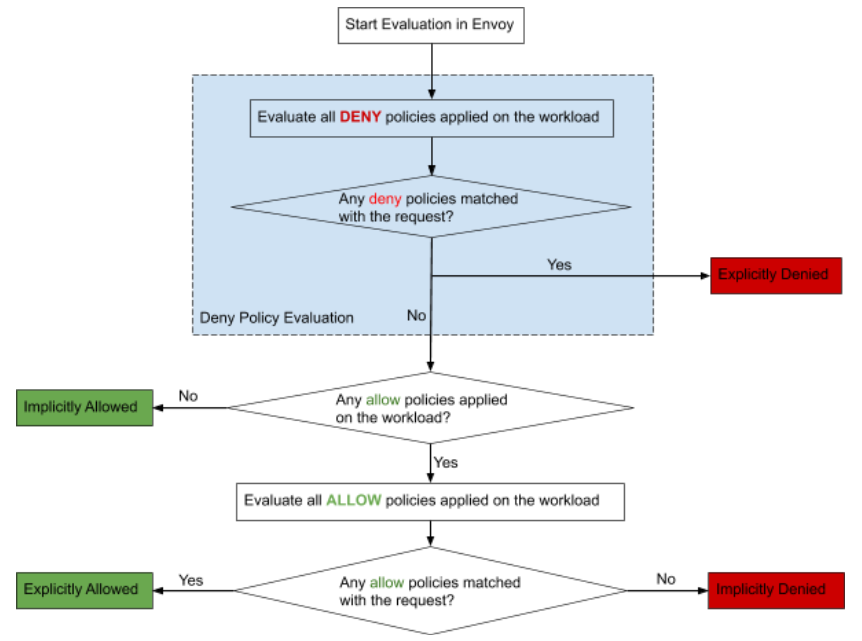
\includegraphics[width=0.75\textwidth]{chapters/images/chp3/env-eval.png}
    \caption{Request evaluation in Envoy}
    \label{fig:env-eval}
\end{figure}

\noindent As it can be seen, the evaluation checks the DENY policies first, denying explicitly if a match occurs. Then, if no DENY policy and no ALLOW policy is defined, the request is implicitly allowed. Finally, if only the ALLOW policies are available, it depends on wether a match occurs or not. If it occurs, then the request is explicitly allowed. If it does not occurs, the request is implicitly denied.
The RBAC configuration file is defined by the documentation \cite{v2api} as follows:

\begin{lstlisting}
action: ALLOW
policies:
  "service-admin":
    permissions:
      - any: true
    principals:
      - authenticated:
          principal_name:
            exact: "cluster.local/ns/default/sa/admin"
      - authenticated:
          principal_name:
            exact: "cluster.local/ns/default/sa/superuser"
  "product-viewer":
    permissions:
        - and_rules:
            rules:
              - header: { name: ":method", exact_match: "GET" }
              - url_path:
                  path: { prefix: "/products" }
              - or_rules:
                  rules:
                    - destination_port: 80
                    - destination_port: 443
    principals:
      - any: true
\end{lstlisting}

\noindent Where in the example is defined a configuration to ALLOW two policies named "service-admin" and "product-viewer".

The RBAC configuration file is built starting from the Internal Model, generated in the same \texttt{model.go}, but using another function:
\begin{lstlisting}[title=\href{https://github.com/istio/istio/blob/4e6e7f49375d84bb35ee614c6b7d38b6c2fd3e7b/pilot/pkg/security/authz/model/model.go\#L167-L196}{GitHub permalink}]
func (m Model) Generate(forTCP, forDeny bool) (*rbacpb.Policy, error)
\end{lstlisting}

\noindent This function generates RBAC Policies, that are divided in two RBAC configurations: one for the DENY action and one for the ALLOW action. In Fig.~\ref{fig:rbac-filter} is shown a schematic example of the translation from the \texttt{AuthorizationPolicy} in Istio API, passing through the Internal Model (Pilot) and saved in Envoy using Envoy API, building a chain of filters used when a request is received.

\begin{figure}[ht]
    \centering
    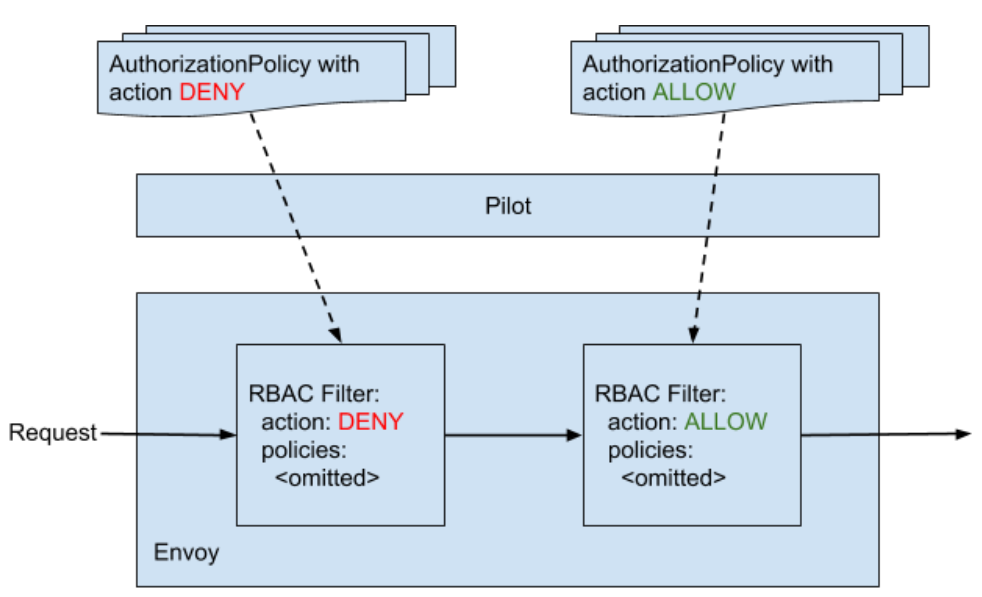
\includegraphics[width=0.9\textwidth]{chapters/images/chp3/rbac-filter.png}
    \caption{Schematic translation of Istio API to Envoy API (actual)}
    \label{fig:rbac-filter}
\end{figure}

At runtime, the first RBAC filter will evaluate the deny policy first which in turn gives the Istio authorization policy with action DENY higher priority than the allow policies.
The drawback is that it adds slightly more processing and memory usage because of the two filter instances. However, the majority time and memory are used for the policy evaluation.
The other drawback is it makes the metrics and logging a little hard to understand as the two filters share the same filter name.

An improvement could be to support mixing allow and deny policies with precedence in the same filter configuration. As shown in Fig.~\ref{fig:rbac-filter2}, Pilot converts the Istio authorization policy to one RBAC filter in Envoy. The RBAC filter is configured with both deny policy and allow policy. The order of the policies field now matters because a policy evaluated earlier takes precedence over the policies evaluated later.

This should be the long term solution, since it slightly decreases the processing and memory usage while simplifying metric and logging.


\begin{figure}[ht]
    \centering
    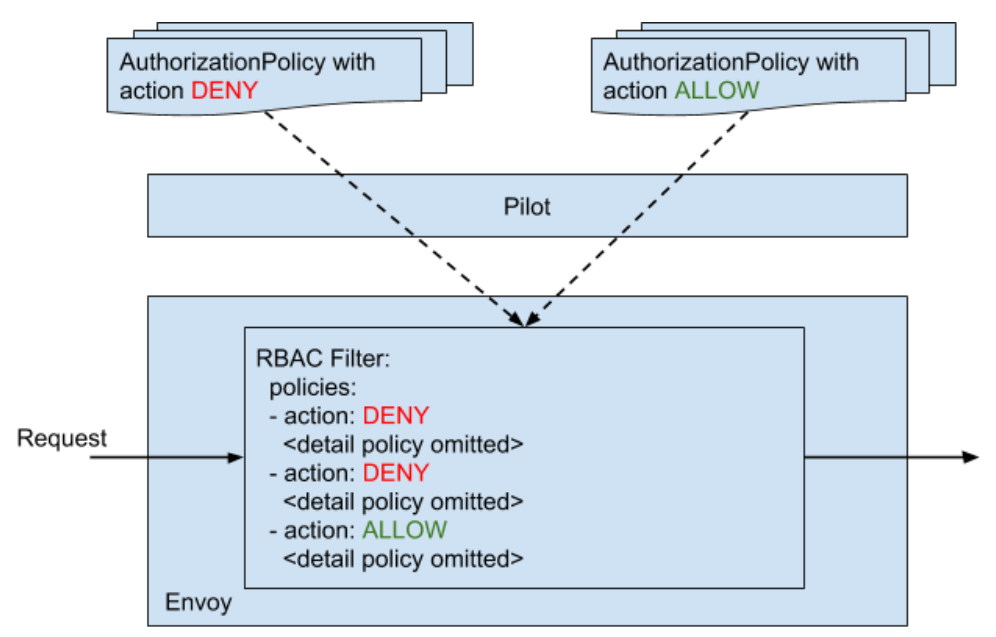
\includegraphics[width=0.92\textwidth]{chapters/images/chp3/rbac-filter2.png}
    \caption{Schematic translation of Istio API to Envoy API (proposed)}
    \label{fig:rbac-filter2}
\end{figure}

\subsection{Policies injection and use in Envoy}
The model is now defined. In order to effectively build the RBAC configuration and inject it into Envoy, a \texttt{builder.go} is used. This script takes the model and the \texttt{AuthorizationPolicy} and returns the RBAC configuration directly in the interested Envoy Proxy. In order to do so, two build funcions are used (one for TCP and one for HTTP):


\begin{lstlisting}[title=\href{https://github.com/istio/istio/blob/4e6e7f49375d84bb35ee614c6b7d38b6c2fd3e7b/pilot/pkg/security/authz/builder/builder.go\#L62-L92}{GitHub permalink}]
func (b Builder) BuildHTTP() []*httppb.HttpFilter
func (b Builder) BuildTCP() []*tcppb.Filter
\end{lstlisting}

\noindent They use a common build function (defined later on) that iterates over the policies and generates an RBAC Rule, that is wrapped in a HTTP or TCP filter based on the current need.

When Envoy receives a request, based on wether the drequest is HTTP or TCP, it enables the corresponding callback in order to ALLOW or DENY the request. For example, a TCP request is managed by this function \cite{envoycode}:

\begin{lstlisting}[title=\href{https://github.com/envoyproxy/envoy/blob/e9207f4f5e93fcec603cf4949763829010836ae2/source/extensions/filters/network/rbac/rbac_filter.cc\#L22-L63}{GitHub permalink}]
Network::FilterStatus RoleBasedAccessControlFilter::onData(Buffer::Instance&, bool)
\end{lstlisting}

That returns the \texttt{Network::FilterStatus}, representing an approval or not.

One of the key benefits of the alpha and beta authorization policy that makes it really useful is the support of authenticated identities. The authenticated identities could either come from mTLS or from the JWT token, as previously discussed.
For example, the following beta policy allows requests based on both the service account from mTLS and the JWT token on the request at the same time:

\begin{lstlisting}

apiVersion: security.istio.io/v1beta1
kind: AuthorizationPolicy
metadata:
 name: httpbin
spec:
 rules:
 - from:
   - source:
       principals: ["cluster.local/ns/default/sa/sleep"]
   to:
   - operation:
       methods: ["POST"]
       paths: ["/upload"]
   when:
   - key: request.auth.claims[iss]
     values: ["https://accounts.google.com"]

\end{lstlisting}

\noindent Namely: \textit{policy “httpbin” allows "cluster.local/ns/default/sa/sleep" to POST on path “/upload” when the request has a valid JWT token issued by "https://accounts.google.com"}. The following diagram in Fig.~\ref{fig:authn-authz} describes how the authenticated attributes get passed to the Envoy RBAC filter.

\begin{figure}[ht]
    \centering
    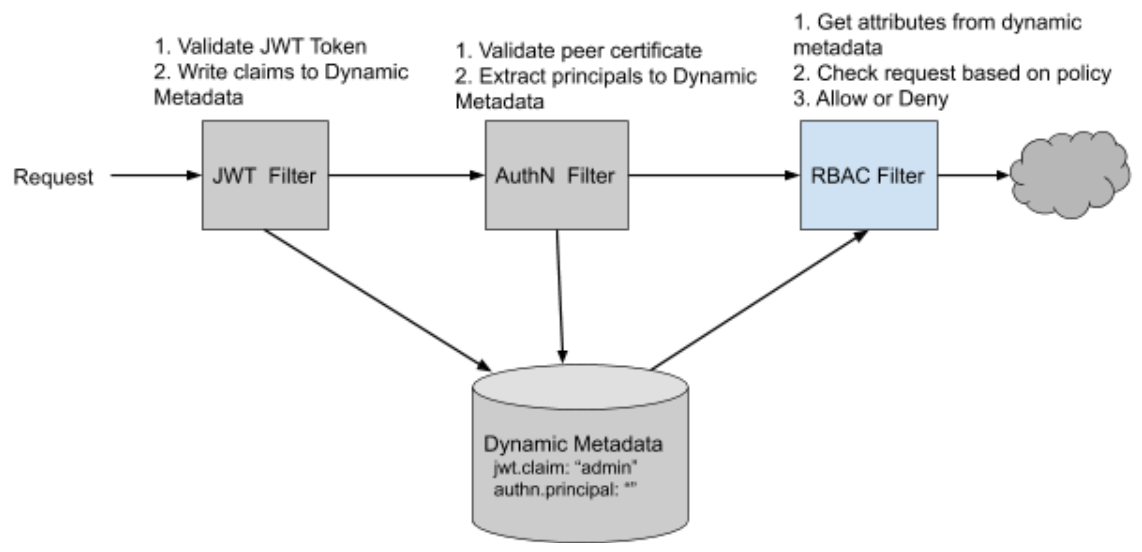
\includegraphics[width=0.92\textwidth]{chapters/images/chp3/authn-authz-ex.png}
    \caption{Schematic representation of authenticated attributes transfer to RBAC by Envoy's Dynamic Metadata}
    \label{fig:authn-authz}
\end{figure}

\begin{enumerate}
    \item JWT filter validates the JWT token on the request and extracts the claims and write it to the dynamic metadata in Envoy.
    \item Istio AuthN filter checks the claims written by JWT filter and also checks the principal of the peer certificates (when mTLS is used) and extract the corresponding attributes based on the Authentication Policy and write it to the dynamic metadata.
    \item RBAC Filter reads from the dynamic metadata to get the authenticated attributes for the access control enforcement.
\end{enumerate}

\noindent The use of Envoy's Dynamic Metadata to pass the generated identities between authentication and authorization at runtime is a clever choice that enhance the security features of Istio.
